\documentclass[11pt]{article}

\usepackage[margin=1in]{geometry}
\usepackage{amsmath,amssymb}
\usepackage{newtxtext,newtxmath}
\usepackage{graphicx}
\usepackage{booktabs}
\usepackage{caption}
\usepackage{subcaption}
\usepackage[dvipsnames]{xcolor}
\usepackage[colorlinks=true,allcolors=NavyBlue]{hyperref}
\usepackage{titlesec}
\usepackage{authblk}
\usepackage{listings}

% Verbatim prompt blocks: wrap long lines rather than run into the margin.
\lstdefinestyle{prompt}{
  basicstyle=\ttfamily\footnotesize,
  breaklines=true,
  breakatwhitespace=false,
  postbreak=\mbox{\textcolor{gray}{$\hookrightarrow$}\space},
  columns=flexible,
  keepspaces=true,
  showstringspaces=false,
  frame=leftline,
  framesep=8pt,
  rulecolor=\color{gray!45},
  xleftmargin=10pt,
  aboveskip=10pt, belowskip=10pt,
}

\captionsetup{font=small,labelfont=bf,skip=6pt}
\titleformat{\section}{\large\bfseries}{\thesection}{0.6em}{}
\titleformat{\subsection}{\normalsize\bfseries}{\thesubsection}{0.6em}{}
\setlength{\parskip}{2pt}

\title{\bfseries Discovery or Recall? A Controlled Test of\\
Language-Model-Driven Evolutionary Search}

\author[ ]{Cheng-You Ho}
\affil[ ]{\normalsize\texttt{}}
\date{}

\begin{document}
\maketitle

\begin{abstract}
\noindent
Evolutionary search driven by large language models is increasingly reported to
``discover'' the structure of a problem, but the evidence for discovery is rarely
separated from the possibility that the structure was supplied to the model in
advance. We encountered this directly. An in-house run appeared to show that
evolutionary search independently found the eight winning lines of tic-tac-toe
and built them into a quantum circuit. An audit of that run showed the winning
lines were listed verbatim in the starter code the model was shown, the task was
named three times in the instructions, and the proposer models know the game from
pretraining. We therefore re-ran the identical search with the answer removed:
no task name, no geometric constants, and a secret relabelling of the nine qubits
that makes the winning lines geometrically meaningless in the coordinates the
model works in. Two of the eight relabelled lines carry no hardware connection at
all, so they can only be found from the accuracy signal, which gives a test that
prior knowledge cannot pass. The contrast is stark. With the answer supplied,
every one of 916 three-qubit gates placed across all successful circuits landed on
a winning line, all eight lines appeared by generation~5, and both
connection-free lines were found. With the answer hidden, three proposers reached
39\%, 0\%, and 7.4\%, none found either connection-free line, and the best circuit
of all used no winning line whatsoever while matching the leaked run's accuracy.
The models' own written rationales settle the mechanism. The one proposer that
reconstructed the domain, correctly naming ``the eight winning lines of a 3x3
board'', placed all eight of its gates on the lines of an \emph{unpermuted} board,
scored below its own earlier attempts, and abandoned the idea. That is recall
being falsified by measurement, not discovery. We also show that the natural
significance test overstates the evidence by eleven orders of magnitude, because
six of the eight winning lines are exactly the triples carrying two hardware
links, so a mundane preference for well-connected qubits mimics discovery. A
second experiment locates what the search can do. On a task whose answer is a
symmetry rather than a convention, and where no symmetry is named anywhere, the
same model derived permutation invariance from the observation that the 28 input
features are exactly the pairs of eight qubits, built an exactly equivariant
circuit at generation 33, and raised test accuracy from 86.7\% to 96.0\% while
cutting parameters from 146 to 26. A third experiment shows how narrow that
capability is. We deleted the one sentence stating that the features are qubit
pairs and changed nothing else, including the reward. Across three proposer
models running 80 generations each, no arm ever built an equivariant circuit and
test accuracy stalled six points lower, at 89 to 90\%. The stated premise was
doing the work, not the search. Rerunning the hidden-answer motif task at the
same 80 generations changed nothing either: usage stayed at or below chance, and
the gates that were placed concentrated on the diagonals of an unpermuted board,
which the relabelling had made wrong. These systems perform one deduction from
what they are shown, and measurement corrects them when it is wrong. They do not
recover the premise itself from the score.
\end{abstract}

\section{The problem}

A recurring claim about evolutionary search driven by large language models is
that it recovers the underlying structure of a problem without being told what
that structure is. The claim matters because it separates two very different
capabilities. A system that rediscovers known structure is a search procedure
with a useful prior. A system that discovers structure nobody supplied is a
scientific instrument. Distinguishing them requires knowing exactly what the
model was shown, and that accounting is usually absent.

The distinction is easy to lose because language models carry enormous prior
knowledge. If a search is run on a task the model already understands, and the
task description or the starter code mentions the relevant structure, then the
model can emit that structure immediately and the search will appear to have
found it. The generational trace will look like discovery even though no search
was required. Nothing in a standard experimental report separates the two cases.

This paper reports a controlled test of that distinction on two concrete tasks,
and a negative result on both. The test is to remove what the model was shown and
rerun. Two of our own runs appeared to show discovery, of a motif in one case and
of a symmetry in the other; in both, removing a single piece of supplied
information removed the result. The motif case is developed first
(Sections~\ref{sec:task} to~\ref{sec:results}), because it has a decisive
sub-test that no statistic can argue with, and the symmetry case follows
(Sections~\ref{sec:sym} and~\ref{sec:zcsym}), because it is where we were wrong
ourselves.

\section{The task, and the terms we need}
\label{sec:task}

\paragraph{The classification problem.}
The task is taken from a standard benchmark in quantum machine learning: classify
a tic-tac-toe board position into one of three outcomes. A board has nine cells,
each empty, a cross, or a circle, encoded as $-1$, $0$, or $+1$. The classifier
must output which of three classes the position belongs to.

\paragraph{Qubits and circuits.}
A \emph{qubit} is a quantum bit. This task uses nine, one per board cell. A
\emph{quantum circuit} is an ordered list of operations applied to those qubits.
The circuit is the object being searched: everything else in the pipeline, that
is the data, the encoding, the training loop, and the readout, is fixed. A
circuit contains \emph{single-qubit gates}, which rotate one qubit,
\emph{two-qubit gates}, which couple a pair, and \emph{three-qubit gates}, which
couple a group of three at once. The search chooses which gates to use and which
qubits they act on.

\paragraph{Triples.}
A \emph{triple} is a set of three qubits joined by a three-qubit gate. From nine
qubits there are $\binom{9}{3} = 84$ possible triples. Which triples the search
selects is the quantity of interest throughout this paper.

\paragraph{Winning lines.}
The eight \emph{winning lines} are the three rows, three columns, and two
diagonals of the board. They are the structure that actually determines the
answer: whether a position is a win is entirely a statement about these eight
triples. A circuit that couples qubits along winning lines has latched onto the
real structure of the task. Figure~\ref{fig:task}(b) shows them.

\paragraph{Hardware connectivity, and why it takes this particular form.}
Real quantum processors cannot couple arbitrary pairs of qubits, because a
two-qubit gate requires the two qubits to be physically adjacent on the chip.
Following the benchmark, we lay the nine qubits out as a $3\times3$ grid and
permit a two-qubit gate only between cells that are immediate neighbours
horizontally or vertically. That rule gives exactly twelve permitted
\emph{pairs}, shown in Figure~\ref{fig:task}(c), and it is the natural topology
for a planar chip: diagonal neighbours are further apart and are not wired.
This list is shown to the model, because it constrains which circuits are legal.
Three-qubit gates are exempt and may act on any triple, so the search is free to
place them anywhere, which is what makes their placement informative.

\paragraph{A structural asymmetry that matters throughout.}
Because the connectivity is exactly grid adjacency, the eight winning lines split
into two kinds. Each of the three rows and three columns is a straight two-step
walk along the grid, so each contains exactly two permitted pairs. Each of the two
diagonals steps diagonally twice, so each contains \emph{no} permitted pair at
all. Rows and columns are therefore visible in the wiring the model is shown:
they are among the connected paths. The two diagonals are invisible in it.
This asymmetry is not a design choice we made, it falls out of putting a
$3\times3$ game on a grid-connected chip, and it turns out to govern both the
statistics (Section~\ref{sec:null}) and what the models actually do
(Section~\ref{sec:results}).

\paragraph{The search procedure.}
We use ShinkaEvolve, an evolutionary loop in which a language model proposes
edits to a program. Each proposal is a modified circuit specification, which is
then trained and scored. Higher-scoring circuits are more likely to be selected
as parents for further edits. One \emph{generation} is one proposed circuit,
evaluated. The score combines validation accuracy, the train-test gap, the loss,
and parameter economy.

\begin{figure}[t]
\centering
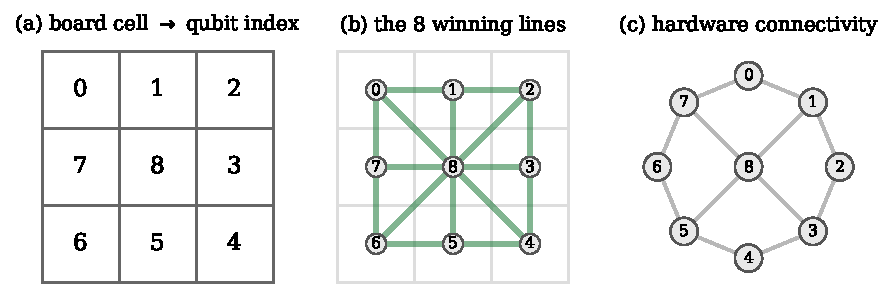
\includegraphics[width=\textwidth]{figs/fig_task.pdf}
\caption{The task and its vocabulary. (a) The nine board cells are mapped to nine
qubits; the benchmark uses a ring-plus-centre labelling, with the perimeter
numbered $0$ to $7$ and the centre $8$. (b) The eight winning lines, the structure
that determines the label. (c) The twelve hardware-permitted qubit pairs; only
these may carry a two-qubit gate.}
\label{fig:task}
\end{figure}

\section{An earlier run that appears to show discovery}
\label{sec:leaky}

We ran this search for 100 generations with a bandit over three proposer models
(Claude Haiku 4.5, GPT-5-mini, and Gemini 3 Flash). The outcome looked like a
clean discovery result. The best circuit, found at generation 77, reached 82.7\%
validation accuracy and 78.2\% test accuracy using only 78 parameters, and it
placed all twelve of its three-qubit gates on winning lines, covering all eight
lines. Across the whole run the pattern was not merely strong but absolute: of
the 916 three-qubit gates placed by all 87 successful circuits, \emph{every
single one} landed on a winning line. All eight lines were already present by
generation~5.

That last observation is what undermines the result. A search that must discover
structure does not converge on all eight members of a 84-element hypothesis space
within five proposals, and it does not achieve a 916 out of 916 hit rate without a
single exploratory error. Perfect performance from the outset is the signature of
transcription, not search.

An audit confirmed it. Three channels supplied the answer. First, the starter
program shown to the model defined the constants \texttt{WIN\_LINES},
\texttt{CORNERS}, and \texttt{CENTER} explicitly, together with an ASCII diagram
of the board, all located above the editable region and therefore included in the
model's context in full. Second, the instructions named tic-tac-toe three times
and described the board geometry. Third, the proposer models know the game from
pretraining regardless of what the prompt says.

The circuit itself carries the fingerprints. The best circuit's parameters are
named \texttt{zzz\_rows}, \texttt{zzz\_cols}, \texttt{zzz\_diags},
\texttt{rot\_corners}, \texttt{rot\_edges}, \texttt{ry\_center},
\texttt{ccrz\_diag}, and \texttt{crz\_ring}. The model was not manipulating
qubit indices, it was reasoning in the semantics of the game, and it tied all
three rows to a single shared parameter, which is the correct symmetry of
tic-tac-toe and not something inferable from an accuracy signal in 77
generations. For comparison, circuits from the anonymised runs below name their
parameters \texttt{zzz\_023} and \texttt{crx\_02}, by coordinate only.

\paragraph{What supplying the motif is worth.}
The value of the motif is established independently, which makes the leaky run's
behaviour easier to interpret. Baumann and
Linnhoff-Popien~\cite{baumann2026} study this task with nine qubits, three
classes, the same rim-plus-centre connectivity, and the same eight winning triples
as the decisive motif. They report roughly 0.63 test accuracy for a
non-symmetric baseline, roughly 0.69 once $D_4$ equivariance is imposed, and
roughly 0.80 once gates aligned to the winning lines are added, and they conclude
that effective circuits need a ``task-informed choice of trainable
interactions''. That is the motif being supplied by a designer, deliberately and
with the reasoning stated. Our leaky run arrived at the same design without
anyone deciding to supply it, reaching 78.2\% test accuracy, and the run was then
read as having discovered what the other work had assumed. The two are the same
experiment under different labels.

\section{The anonymised protocol}
\label{sec:anon}

We rebuilt the task so that prior knowledge cannot substitute for search, holding
everything else fixed. Four changes were made. The instructions never mention
tic-tac-toe, boards, rows, columns, corners, or centres, and describe only an
abstract nine-input, three-class problem. The starter program contains no
geometric constants and no diagram. Labels are precomputed offline, so no
scoring rule in the visible code reveals the structure. Most importantly, we
applied a secret permutation to the qubit labels, drawn once with a fixed seed
and baked into the data, the readout, and the connectivity list.

The full task message sent to the proposer is reproduced verbatim in
Appendix~\ref{app:prompts}, alongside the leaked seed constants from the original
run, so that the difference between the two conditions can be checked directly
rather than taken on trust.

The permutation is what makes the test work. Under relabelling the winning lines
remain exactly as predictive as before, so the accuracy signal is unchanged, but
they are no longer rows or columns of anything the model can see.
Figure~\ref{fig:anonymize} shows the effect: what is an obvious geometric family
in board coordinates becomes an unremarkable scatter of triples in qubit
coordinates. A model recalling tic-tac-toe would place gates on the original
rows and columns, which are now wrong.

\begin{figure}[t]
\centering
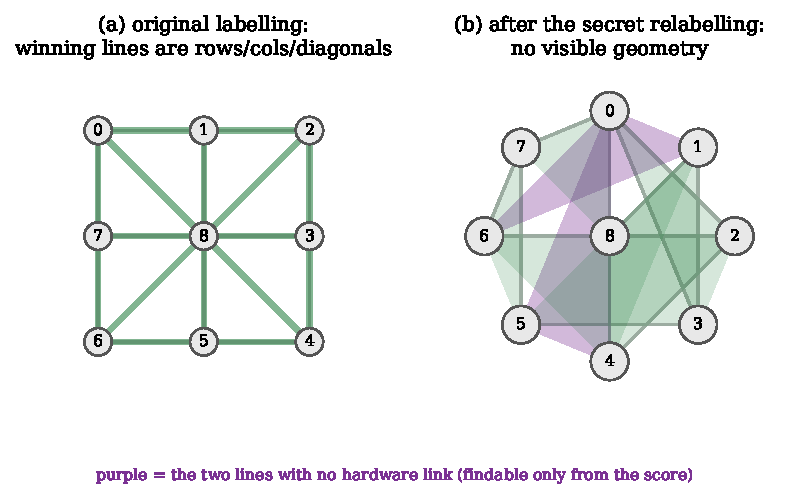
\includegraphics[width=0.86\textwidth]{figs/fig_anonymize.pdf}
\caption{What anonymisation does. (a) In the original labelling the eight winning
lines are visibly rows, columns, and diagonals. (b) After the secret relabelling
the same eight triples, now drawn on the hardware graph the model actually sees,
have no visible geometry. Purple marks the two lines containing no hardware link,
which cannot be reached by following structural hints.}
\label{fig:anonymize}
\end{figure}

\paragraph{The decisive sub-test.}
The two diagonals, which after relabelling are the triples $(0,1,6)$ and
$(0,4,5)$, contain no hardware-permitted pair among their three qubits. Nothing
in the visible problem points at them. They are reachable only by noticing that
circuits using them score better. We designate these the \emph{hidden lines}, and
finding one is the strongest available evidence of genuine, score-driven
discovery.

\paragraph{Runs.}
We ran three arms that differ only in the proposer model: Claude Haiku 4.5,
Claude Sonnet 5, and GPT-5.6-sol. Each ran for 30 generations under an identical
protocol and an identical evaluation budget.

\section{What should count as chance}
\label{sec:null}

The obvious baseline is that a circuit placing triples at random would hit a
winning line with probability $8/84 = 0.095$. We argue this baseline is wrong,
and that using it substantially overstates the evidence for discovery.

The winning lines are not distributed uniformly with respect to the hardware
connectivity that the model is shown. Sorting all 84 triples by how many of their
three pairs are hardware links gives the structure in
Figure~\ref{fig:strata}: of the 22 triples containing two hardware links, six are
winning lines, a rate of $0.273$; of the 40 triples containing exactly one link,
\emph{none} is a winning line; of the 22 containing none, two are.

The consequence is direct. A proposer that simply favours well-connected triples,
for ordinary engineering reasons and with no insight into the task, will land on
winning lines about 27\% of the time. Any test against the uniform 9.5\% baseline
will report such a proposer as making a highly significant discovery. We
therefore report significance against both baselines, and treat the
connectivity-matched figure of $0.273$ as the honest one.

\begin{figure}[t]
\centering
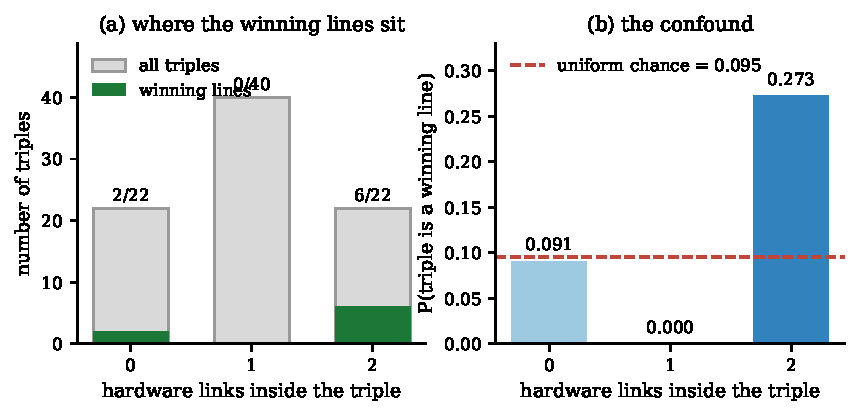
\includegraphics[width=0.92\textwidth]{figs/fig_strata.pdf}
\caption{Why the naive baseline is too generous. (a) The 84 triples grouped by how
many hardware links they contain, with winning lines highlighted; six of the eight
sit in the two-link group. (b) The resulting hit rate per group. A preference for
well-connected triples alone yields $0.273$, nearly three times the uniform
baseline of $0.095$.}
\label{fig:strata}
\end{figure}

\section{Results}
\label{sec:results}

\subsection{Motif usage collapses once the answer is hidden}

Table~\ref{tab:main} gives the comparison. The leaky run placed 916 of 916 gates
on winning lines. The three anonymised arms placed 35 of 89 (39\%), 0 of 46
(0\%), and 7 of 95 (7.4\%). The last figure is \emph{below} the uniform chance
level of 9.5\%. Three runs of an identical protocol, differing only in which
model proposes, produced a moderate effect, no effect, and a slightly
below-chance effect.

\begin{table}[t]
\centering
\small
\caption{Motif usage with the answer supplied and with it hidden. ``Gates on
lines'' counts every three-qubit gate placed by every successful circuit.
$p_{\text{unif}}$ tests against the uniform baseline $0.095$; $p_{\text{conn}}$
tests against the connectivity-matched baseline $0.273$.}
\label{tab:main}
\begin{tabular}{lcccc}
\toprule
& \textbf{Leaky} & \textbf{Haiku 4.5} & \textbf{Sonnet 5} & \textbf{GPT-5.6-sol} \\
& answer given & hidden & hidden & hidden \\
\midrule
Generations & 100 & 30 & 30 & 30 \\
Gates on lines & 916/916 (100\%) & 35/89 (39\%) & 0/46 (0\%) & 7/95 (7.4\%) \\
$p_{\text{unif}}$ & ${\sim}10^{-935}$ & $6.7\times10^{-14}$ & $1.00$ & $0.81$ \\
$p_{\text{conn}}$ & ${\sim}10^{-517}$ & $9.1\times10^{-3}$ & $1.00$ & $1.00$ \\
Distinct lines found & 8/8 & 3/8 & 0/8 & 0/8 \\
\textbf{Hidden lines found} & \textbf{2/2} & \textbf{0/2} & \textbf{0/2} & \textbf{0/2} \\
First line at generation & 5 & 2 & never & never \\
Proposals naming the game & 92\% & 10\% & 27\% & 30\% \\
Best validation accuracy & 82.7\% & 67.7\% & 72.0\% & \textbf{82.3\%} \\
Best test accuracy & 78.2\% & 65.5\% & 65.7\% & \textbf{77.8\%} \\
Parameters in best circuit & 78 & 180 & 186 & 108 \\
\bottomrule
\end{tabular}
\end{table}

\subsection{Most of the surviving effect is the connectivity confound}

The Haiku arm's 39\% is significant against the uniform baseline at
$p = 6.7\times10^{-14}$, which reads as decisive. It is not. That arm placed 69 of
its 89 gates, or 78\%, on two-link triples, against the 26\% expected if it were
choosing blindly, so it had a strong independent preference for well-connected
triples. Measured against the connectivity-matched baseline the effect shrinks to
$p = 9.1\times10^{-3}$, weaker by eleven orders of magnitude. Restricting
attention to the single best circuit, which places three of five gates on lines,
the effect is not significant at all ($p = 0.13$). A real but modest residual
enrichment remains; a discovery does not.

\subsection{Neither model found a hidden line}

Both anonymised arms found zero of the two hidden lines
(Figure~\ref{fig:summary}(c)). Every winning line either arm touched was one
carrying hardware links, and therefore reachable by following visible structure.
The three lines the Haiku arm found were all of this kind. The two lines that
require the accuracy signal alone were never found. The leaky run, by contrast,
found both, which is expected because it was given them.

\subsection{The best circuit overall used no winning line at all}

The GPT-5.6-sol arm reached 82.3\% validation and 77.8\% test accuracy, matching
the leaky run's 82.7\% and 78.2\% to within a fraction of a point, using 108
parameters against the leaky run's 78. It did so while placing \emph{zero} of its
four three-qubit gates on winning lines, and 7 of 95 across the whole run, below
the uniform chance level. The Sonnet arm shows the same pattern more weakly:
72.0\% validation accuracy with no gates on winning lines, and 28 of its 46 gates
on one-link triples, which by construction can never be winning lines.

This is the result that most damages the original claim. The motif is not
necessary. An arm that never used a winning line matched the accuracy of the arm
that was handed all eight of them. Whatever the leaky run's perfect motif coverage
bought, it was not accuracy unobtainable by other means, so the coverage cannot be
read as evidence that the search had found the one right structure.

\subsection{How the proposers reason, and a direct test of recall}
\label{sec:reasoning}

Each proposal carries a natural-language description in which the model explains
what it is changing and why. Reading these gives a view of the search that the
statistics cannot provide, and it settles the question of whether anonymisation
actually worked.

\paragraph{The leaky run reasons in the language of the game throughout.}
Of its 90 proposals, 83 (92\%) use game vocabulary, beginning with the very first
edit at generation~5, whose description already refers to ``tic-tac-toe'',
``winning line'', ``corner'' and ``center''. Proposals carry names such as
\texttt{winning\_lines\_zzz\_augmentation}, \texttt{zz\_split\_rowcoldiag\_motif},
and \texttt{symmetry\_shared\_ccrz\_diagonals}. The search was never looking for
the motif; it was engineering around a motif it had been given on the first move.

\paragraph{Anonymisation reduced this sharply but did not eliminate it.}
Game vocabulary appears in 10\% of Haiku's proposals, 27\% of Sonnet's, and 30\%
of GPT-5.6-sol's (Figure~\ref{fig:vocab}). The residue matters: GPT-5.6-sol
reconstructed the task. At generation~9 it wrote that it was aligning its gates to
``the eight winning lines of a 3x3 board'', and at generation~8 it described
sharing ``one parameter shared by all rows and columns, while another is shared by
the two diagonals'', which is the correct symmetry decomposition of the square.
Removing the task name and the constants did not prevent a capable model from
inferring the domain from the shape of the data alone.

\paragraph{What it did with that inference is the decisive measurement.}
A model that has \emph{recalled} tic-tac-toe knows the lines in the standard
layout, but the secret permutation has moved them, so recalled lines should be
wrong. A model that has \emph{discovered} the structure would target the true
lines. These predictions are distinguishable, and the data are unambiguous. At
each of generations 3, 7, 8, 9 and 10, GPT-5.6-sol placed exactly eight
three-qubit gates, and all eight fell on the winning lines of an unpermuted
row-major board. Only one of the eight coincided with a true line, and that
triple, $(2,4,6)$, belongs to both sets by coincidence
(Figure~\ref{fig:recall}(a)).

\paragraph{The score rejected the recalled motif.}
Those five proposals scored between 0.546 and 0.578, well below the 0.725 the same
arm had already reached at generation~5 with an unrelated design
(Figure~\ref{fig:recall}(b)). The model abandoned the idea, and its subsequent
proposals turn to readout-aligned and class-aligned constructions with no
geometric content, ending at 0.734. The evolutionary loop behaved exactly as it
should: a confident, articulate, incorrect hypothesis was proposed, measured, and
discarded on the evidence.

\begin{figure}[t]
\centering
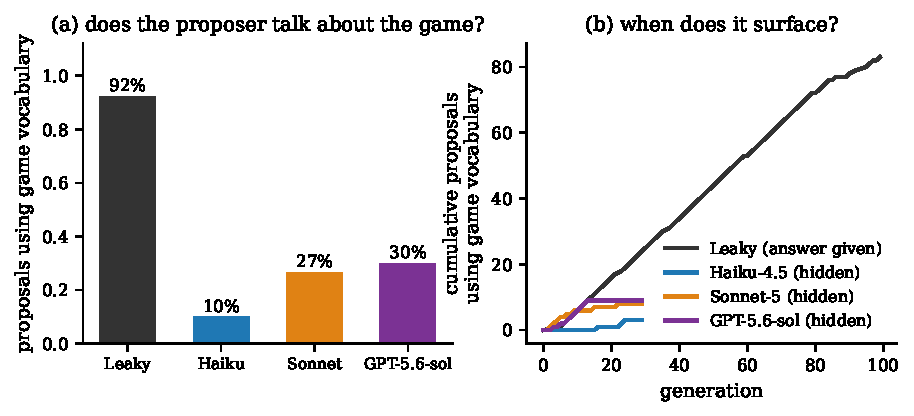
\includegraphics[width=\textwidth]{figs/fig_vocab.pdf}
\caption{Reasoning traces. (a) Share of proposals whose description uses
vocabulary from the underlying game. Anonymisation cuts this from 92\% to between
10\% and 30\%, but does not remove it. (b) Cumulative count over generations; the
leaky run engages the game from its first edit and never stops.}
\label{fig:vocab}
\end{figure}

\begin{figure}[t]
\centering
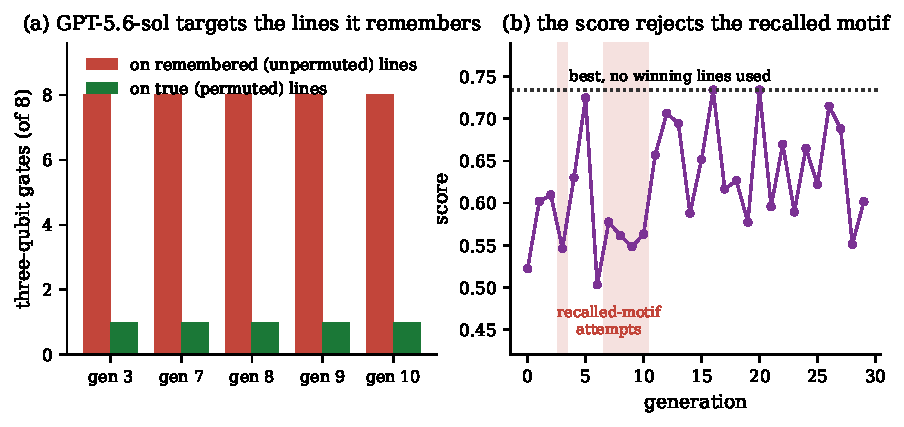
\includegraphics[width=\textwidth]{figs/fig_recall.pdf}
\caption{Recall, not discovery. (a) In the five generations where GPT-5.6-sol
stated it was targeting winning lines, all eight of its gates landed on the lines
of an \emph{unpermuted} board and essentially none on the true permuted lines.
(b) Those attempts (shaded) score below what the arm had already achieved, and
below its eventual best, which uses no winning line at all.}
\label{fig:recall}
\end{figure}

\begin{figure}[t]
\centering
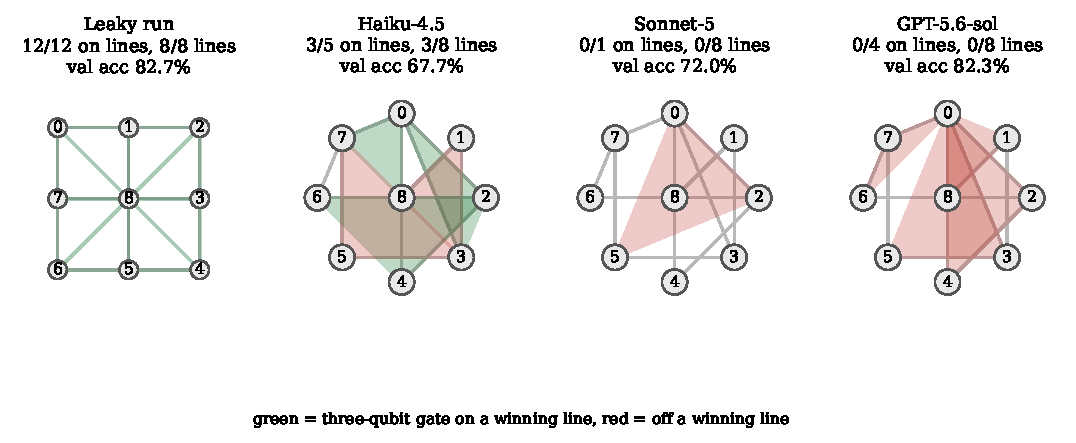
\includegraphics[width=\textwidth]{figs/fig_circuits.pdf}
\caption{The best circuit from each run, drawn as the triples its three-qubit
gates act on. Grey lines are hardware-permitted pairs. The leaky circuit
(left) covers the winning lines exactly and completely. The anonymised circuits
use fewer three-qubit gates, place them partly or entirely off the winning lines,
and reach lower accuracy.}
\label{fig:circuits}
\end{figure}

\begin{figure}[t]
\centering
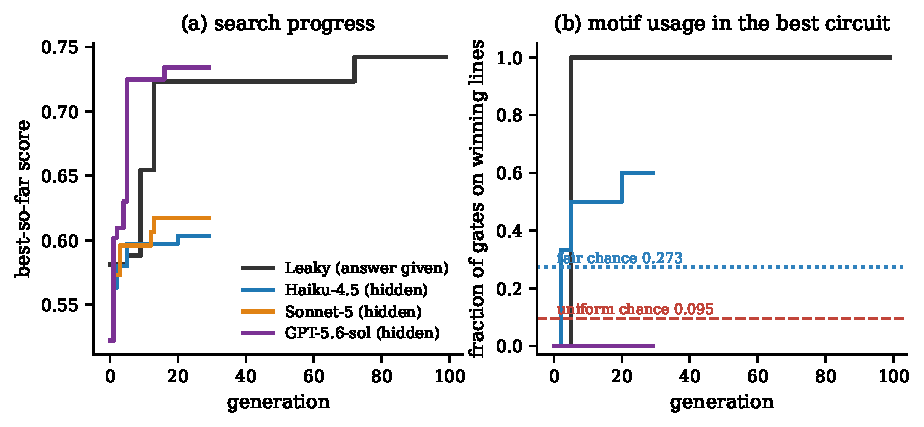
\includegraphics[width=\textwidth]{figs/fig_trajectory.pdf}
\caption{Search trajectories. (a) Best score so far against generation.
(b) Fraction of the best circuit's three-qubit gates lying on winning lines. The
leaky run reaches and holds $1.0$ almost immediately. The anonymised runs
fluctuate near or below the connectivity-matched baseline.}
\label{fig:trajectory}
\end{figure}

\begin{figure}[t]
\centering
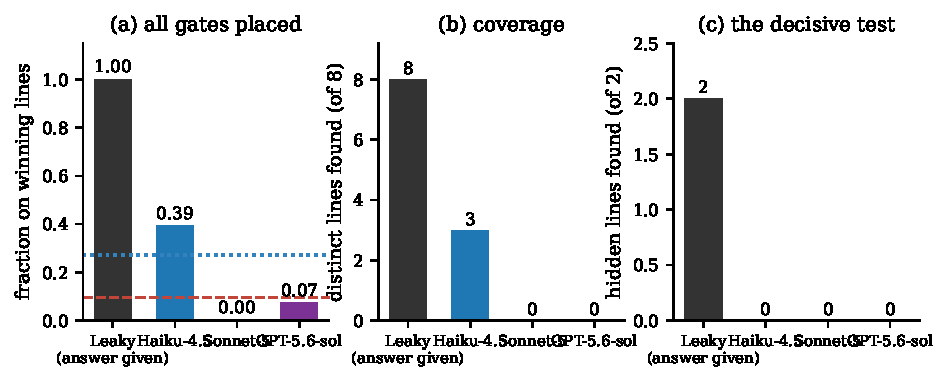
\includegraphics[width=\textwidth]{figs/fig_summary.pdf}
\caption{Summary. (a) Fraction of all placed gates on winning lines, against the
uniform (red dashed) and connectivity-matched (blue dotted) baselines.
(b) Distinct winning lines found. (c) The decisive test: hidden lines found, which
only the run that was given the answer passes.}
\label{fig:summary}
\end{figure}

\subsection{A longer run, with the context removed as well}
\label{sec:zcmotif}

The 30-generation limit above was imposed by budget, so we repeated the
experiment at 80 generations with the remaining context stripped as well. The
anonymised protocol still described the task in the instructions and still showed
a seed program containing the data loading, the encoding and the readout. Here
the instructions state only the qubit count, the legal gate schema, the
parameter-sharing mechanism and what the score rewards, and say explicitly that
the model is not told what the data is. Everything about the pipeline moved into
an imported module, so the visible seed is roughly 55 lines with a docstring that
describes nothing. The secret relabelling is unchanged, so the two hidden lines
remain the decisive test.

Motif usage fell further rather than rising with the longer horizon. Haiku placed
1 of 180 three-qubit gates on a true line, Sonnet 3 of 52, and GPT-5.6-sol 12 of
18. No arm found either hidden line, and none of the three best circuits used a
winning line at all: the best circuits score 0.615, 0.628 and 0.625, against the
leaky run's 0.742.

The GPT-5.6-sol figure of 12 out of 18 is the only enrichment anywhere in the
zero-context data, and it does not survive inspection
(Figure~\ref{fig:zcmotif}). Seven of those twelve placements are the single
triple $(2,4,6)$, repeated down a lineage across seven generations. That triple
is the one member of the true permuted set that is \emph{also} a winning line of
an unpermuted row-major board, the coincidence noted in
Section~\ref{sec:reasoning}. The arm was placing the anti-diagonal it remembered
and being credited for a hit it did not earn. Counting each distinct triple once,
which removes the pseudoreplication of inheritance, gives 3 of 7 on lines, which
is not significant against the connectivity-matched baseline ($p = 0.29$).

The same recalled geometry appears in the arms with no enrichment, where it is
unambiguously wrong. Haiku's most-used triple by a wide margin is $(0,4,8)$, with
56 of its 180 placements, and Sonnet also favours it. That is the main diagonal
of an unpermuted board, and under the relabelling it is not a winning line at
all. Across all three arms the gates concentrate on the two diagonals of the
board the models remember, one of which happens to be right and one of which is
wrong, which is the signature of recall rather than search.

\begin{table}[t]
\centering
\small
\caption{The motif task at 80 generations with the context removed as well.
``Distinct'' counts each triple once however many circuits inherited it.
Compare Table~\ref{tab:main}: the leaky run placed 916 of 916 gates on lines and
found both hidden lines.}
\label{tab:zc}
\begin{tabular}{lccc}
\toprule
& \textbf{Haiku 4.5} & \textbf{Sonnet 5} & \textbf{GPT-5.6-sol} \\
\midrule
Generations & 80 & 80 & 80 \\
Gates on lines & 1/180 (0.6\%) & 3/52 (5.8\%) & 12/18 (67\%) \\
\quad of which the coincidence triple & 1 & 1 & 7 \\
Distinct triples on lines & 1/13 & 2/24 & 3/7 \\
$p_{\text{conn}}$ (distinct) & $0.98$ & $1.00$ & $0.29$ \\
Distinct lines found & 1/8 & 2/8 & 3/8 \\
\textbf{Hidden lines found} & \textbf{0/2} & \textbf{0/2} & \textbf{0/2} \\
Game vocabulary & 5\% & 5\% & 16\% \\
Best score & 0.615 & 0.628 & 0.625 \\
Best test accuracy & 64.2\% & 65.0\% & 62.3\% \\
Lines in best circuit & 0/3 & no triples & no triples \\
\bottomrule
\end{tabular}
\end{table}

\begin{figure}[t]
\centering
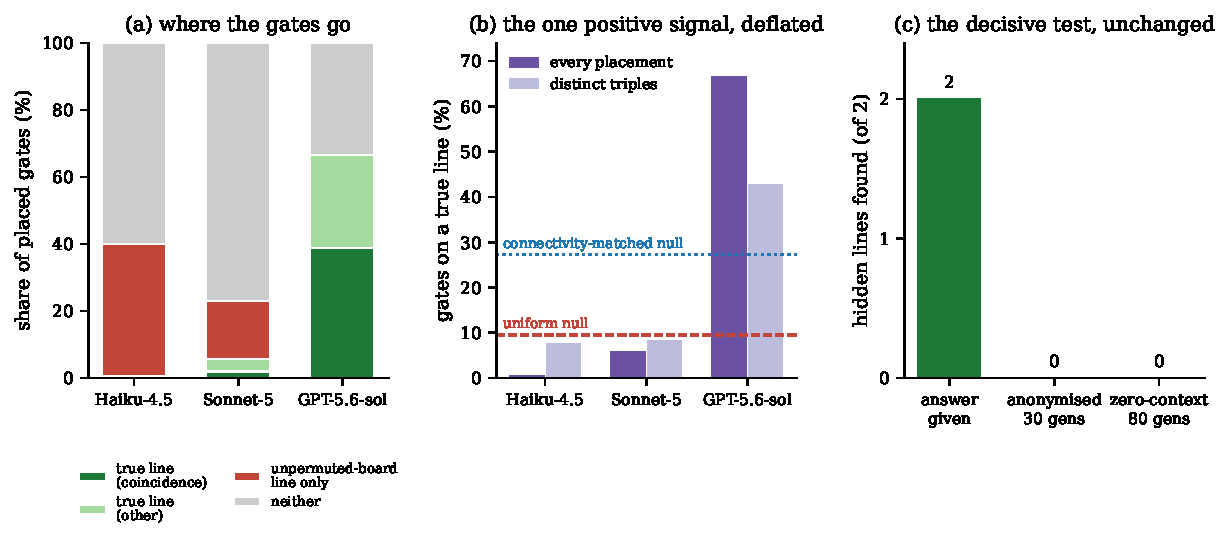
\includegraphics[width=\textwidth]{figs/fig_zc_motif.pdf}
\caption{The zero-context motif runs, 80 generations each. (a) Every three-qubit
gate placed, classified by whether its triple is a true winning line, a winning
line of an unpermuted board only, or neither. (b) The on-line rate counted per
placement and per distinct triple; the one enrichment shrinks below the
connectivity-matched baseline once inherited copies are counted once.
(c) Hidden lines found, which remains zero.}
\label{fig:zcmotif}
\end{figure}

\section{A second test, where the answer is derivable}
\label{sec:sym}

The motif test may be unfair in a specific way. Winning lines are a convention:
you either know tic-tac-toe or you do not, and no amount of staring at permuted
qubit indices will yield them. A symmetry is different. It can in principle be
read off the shape of the data. If the failure above is really about
\emph{derivability} rather than about search, then a target that is derivable
should be found. We had two further runs available to test this, built and
launched independently of the motif work.

\paragraph{Two tasks whose answer is a symmetry.}
The first task classifies networks. Each record lists which of the 28 possible
connections among eight nodes are present, and the label depends only on the
shape of the network, not on which node is called which. Renaming the nodes is
therefore an exact symmetry, and we confirmed this holds in the data: all 815
distinct relabelling-invariant classes carry a single label, covering all 1350
records, and every relabelled copy we could locate kept its label. The second
task classifies quantum states that are all rotationally balanced, a property we
confirmed by computing that every state has total spin exactly zero. Neither
task's instructions or seed program mentions symmetry, invariance, permutation,
spin or any group; we grepped for all of these and found nothing, and both task
messages are reproduced verbatim in Appendix~\ref{app:prompts}. Both tasks also
allow two-qubit gates on any pair, so the connectivity confound of
Section~\ref{sec:null} does not arise.

\paragraph{One thing was stated, and it turned out to be the whole result.}
The tasks do withhold every word for the symmetry, but they do not withhold the
fact the symmetry follows from. The seed program's docstring reads: ``Each
feature $k$ is encoded by the fixed feature map as a two-qubit phase coupling on
the qubit pair \texttt{FEATURE\_PAIRS[k]}.'' That sentence states that the 28
features are the pairs of eight qubits, which is the premise the winning
derivation below runs on. ShinkaEvolve places the entire seed file in the prompt,
so sanitising the instructions alone does not withhold it, which is the same
channel that leaked the winning lines in Section~\ref{sec:leaky}. We only
recognised this after reading the winning rationale, and Section~\ref{sec:zcsym}
reports what happens when the sentence is removed.

\paragraph{Measuring equivariance exactly.}
Shared parameters and uniform gate patterns can be produced by the score's
parameter-economy term alone, so we test the strong property directly: relabel
the eight wires and ask whether the resulting gate multiset, parameter identities
included, is unchanged. We report the fraction of the block preserved under
random relabelling, which is $1.0$ only for an exactly equivariant circuit.

\paragraph{The network task: the search finds the symmetry and the score pays for it.}
GPT-5.6-sol produced its first exactly equivariant circuit at generation~33, in a
proposal it named \texttt{permutation\_equivariant\_ansatz}, whose rationale reads:

\begin{quote}\small
Exploit the likely graph structure of the 28 binary features, which correspond
exactly to all unordered pairs of eight qubits. \ldots\ Replace wire-specific
rotations and the symmetry-breaking ring with a permutation-equivariant block:
rotation parameters are shared across all qubits, and CZ gates cover the complete
graph. This aligns the circuit with relabeling-invariant graph classification.
\end{quote}

The reasoning is a derivation, not a recollection: $28 = \binom{8}{2}$ implies a
graph, a graph label implies relabelling invariance, and relabelling invariance
implies shared rotations on a complete-graph entangler. The run divides sharply
at that generation. Mean equivariance across proposals rises from $0.154$ to
$0.946$, mean score from $0.821$ to $0.932$, and best score from $0.871$ to
$0.948$ (Figure~\ref{fig:symmetry}). The final circuit reaches 96.0\% test
accuracy with 26 parameters against the seed's 86.7\% with 146.

\paragraph{Equivariance orders the arms.}
Across models the ranking is monotone in how symmetric the final circuit is:
GPT-5.6-sol at equivariance $0.96$ and 96.0\% accuracy with 26 parameters,
Haiku~4.5 at $0.66$ and 92.0\% with 38, Sonnet~5 at $0.18$ and 92.0\% with 98,
against the seed at $0.15$ and 86.7\% with 146. Accuracy improves alongside the
parameter reduction, so this is not the parameter-economy term being satisfied on
its own.

\paragraph{The quantum-state task is uninformative.}
All three arms reach 100\% validation and test accuracy by generations 2, 6 and 9
respectively, from a first-proposal score of 0.811. The task saturates before any
design pressure can act, and no arm adopted the rotation-invariant coupling that
the gate set made available. We report it for completeness and draw no conclusion
from it; it needs to be made harder before it can test anything.

\begin{figure}[t]
\centering
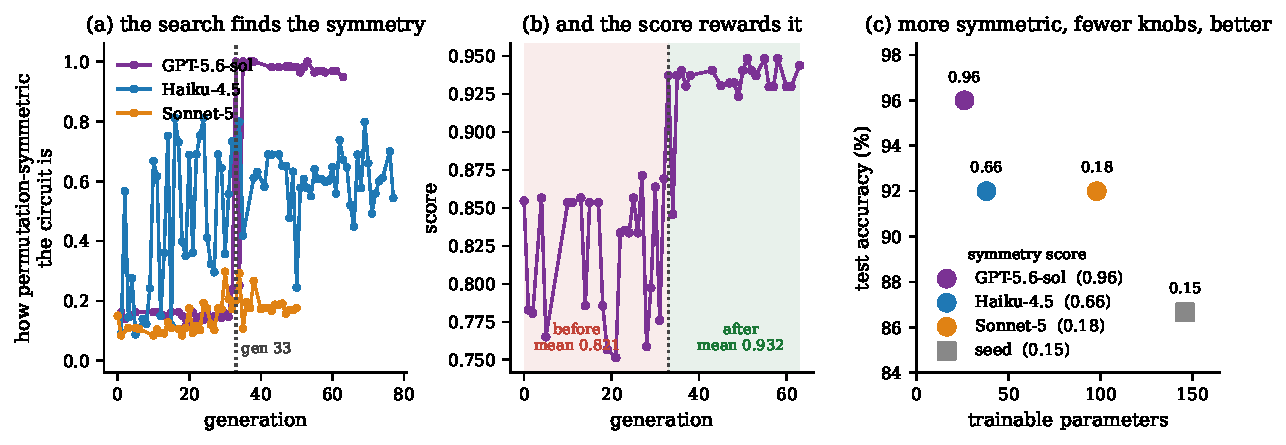
\includegraphics[width=\textwidth]{figs/fig_symmetry.pdf}
\caption{The network task. (a) How symmetric each proposed circuit is, against
generation; GPT-5.6-sol jumps to exact equivariance at generation~33 and stays
there. (b) The score for that arm before and after the same point. (c) Final
circuits: more symmetric circuits use fewer parameters and score higher, with the
seed at lower right.}
\label{fig:symmetry}
\end{figure}

\section{Removing the stated premise removes the result}
\label{sec:zcsym}

The derivation in Section~\ref{sec:sym} begins by asserting that the 28 features
are the unordered pairs of eight qubits, which the seed docstring supplies. That
makes the network result a test of one deductive step from a given premise, not a
test of whether the search can find the premise. We rebuilt the task to remove
it and changed nothing else, including the reward, the data, the gate vocabulary
and the evaluation budget.

\paragraph{What the proposer is left with.}
The instructions state the qubit count, the legal gate schema, the
parameter-sharing mechanism, and what the score rewards, and say explicitly that
the model is not told what the data is or how it is encoded. Everything about
data loading, encoding, readout, training and metrics moved into an imported
module, so the visible seed is roughly 55 lines: a docstring that describes
nothing, the qubit count, the gate vocabulary, the evolve block, and a one-line
delegation. The evaluation script is written to disk for execution and never
shown, so the scoring formula stays hidden. The symmetry is still exactly as
present in the data, and the score still pays for it exactly as much.

\paragraph{No arm found it.}
We ran three proposer models for 80 generations each, more than the 64 the
winning hinted arm had used. Not one produced an exactly equivariant circuit
(Figure~\ref{fig:zerocontext}, Table~\ref{tab:zcsym}). The best circuits of the
GPT-5.6-sol, Haiku and Sonnet arms reach partial equivariance $0.46$, $0.38$ and
$0.09$, against $0.96$ for the hinted GPT arm. Test accuracy stalls at 90.0\%,
89.3\% and 89.0\%, against 96.0\% hinted, using 62, 50 and 122 parameters against
26. Exactness rather than the average is what separates the conditions: the
hinted Haiku arm averaged the same partial equivariance as the hinted GPT arm and
also never reached $1.0$, so a high average measures parameter sharing, and only
the exact test measures the symmetry. The seed is at 86.7\% with 146, so the
zero-context arms did improve on it, by compressing parameters and tuning
topology. They did not find the structure that was worth the other six points.

\paragraph{They proposed symmetry, but the wrong one.}
Ten or eleven proposals per arm use symmetry vocabulary, so the idea was not
absent. What they mean by it is local: sharing rotation angles between even and
odd wires, mirroring a layer, tying a chain back on itself. Names such as
\texttt{parity\_tied\_phase\_ansatz} and \texttt{reflection\_shared\_chain} are
typical, and the best zero-context GPT-5.6-sol proposal explains that it will
``share the initial RY angles by wire parity, replacing eight independent
parameters with two''. Parity sharing is a subgroup of order two. The task's
symmetry is the full $S_8$, of order 40320, and reaching it requires knowing that
the wires are interchangeable nodes of a graph. One proposal in 232 uses the word
``relabel'' at all. The search was doing parameter economy, which the score also
rewards, and never arrived at the hypothesis that the score would have paid much
more for.

\begin{table}[t]
\centering
\small
\caption{The network task with and without the one sentence stating that the 28
features are the pairs of eight qubits. Equivariance is the fraction of the
circuit preserved under a random relabelling of the eight wires, which is $1.0$
only for an exactly equivariant circuit. The data, the reward and the gate
vocabulary are identical across the two conditions.}
\label{tab:zcsym}
\begin{tabular}{lcccccc}
\toprule
& \multicolumn{3}{c}{\textbf{Premise stated}} & \multicolumn{3}{c}{\textbf{Premise removed}} \\
\cmidrule(lr){2-4}\cmidrule(lr){5-7}
& GPT-5.6 & Haiku & Sonnet & GPT-5.6 & Haiku & Sonnet \\
\midrule
Generations & 64 & 78 & 51 & 80 & 80 & 80 \\
\textbf{Exactly equivariant circuits} & \textbf{5} & 0 & 0 & \textbf{0} & \textbf{0} & \textbf{0} \\
First at generation & 33 & never & never & never & never & never \\
Equivariance of best circuit & 0.96 & 0.66 & 0.18 & 0.46 & 0.38 & 0.09 \\
Mean equivariance & 0.53 & 0.53 & 0.15 & 0.32 & 0.36 & 0.14 \\
Test accuracy & \textbf{96.0\%} & 92.0\% & 92.0\% & 90.0\% & 89.3\% & 89.0\% \\
Parameters & \textbf{26} & 38 & 98 & 62 & 50 & 122 \\
\bottomrule
\end{tabular}
\par\vspace{2pt}
{\footnotesize The seed circuit scores 86.7\% with 146 parameters at equivariance $0.15$.}
\end{table}

\begin{figure}[t]
\centering
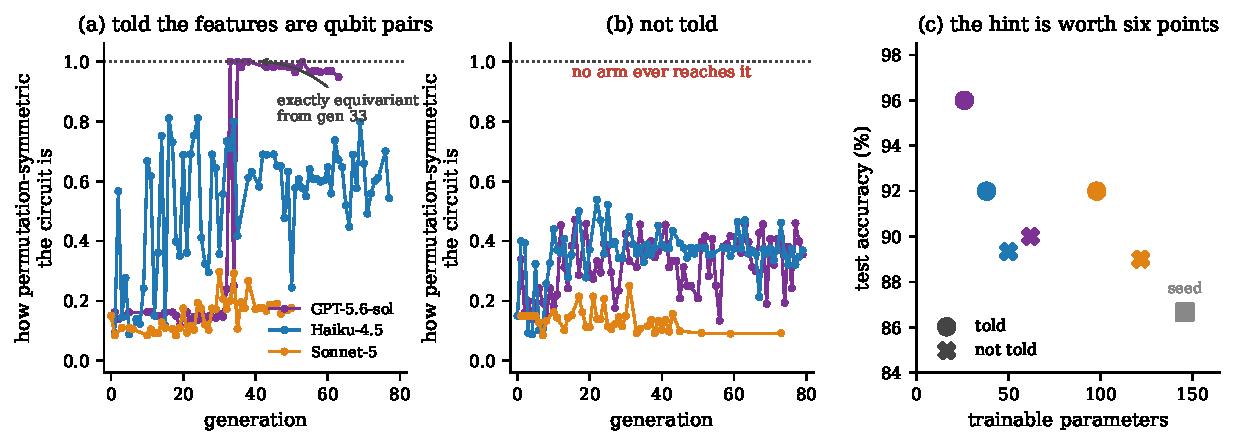
\includegraphics[width=\textwidth]{figs/fig_zerocontext.pdf}
\caption{The network task with and without the sentence stating that the 28
features are qubit pairs. (a) With it: GPT-5.6-sol reaches exact equivariance at
generation~33 and holds it. (b) Without it, at a longer horizon: all three arms
plateau between $0.1$ and $0.5$ and none reaches exact equivariance.
(c) Best circuit of each arm; withholding one sentence costs six points of test
accuracy and doubles to quintuples the parameter count.}
\label{fig:zerocontext}
\end{figure}

\paragraph{The spin task broke in a way worth recording.}
We also rebuilt the quantum-state task, whose earlier saturation made it useless,
by strengthening the parameter-economy term so the score would keep
discriminating down to about four parameters, and by cutting the training set
from 450 records to 24 so that generalisation rather than fit became the binding
constraint. The redesign made the empty circuit optimal. Forty-nine of Sonnet's
70 valid proposals contain no gates at all, and its best-scoring program is one
of them: zero gates, score 0.803, and 100\% test accuracy. Every arm reaches 100\%
test accuracy regardless of what it proposes, which means the fixed feature map
and readout already solve the task and the ansatz contributes nothing. No arm in
any condition, hinted or not, ever tied XX, YY and ZZ on a pair into the
rotationally invariant coupling. This arm tests nothing about discovery, and we
report it because the failure is instructive: raising the weight on parameter
economy in a task the encoder already solves does not create design pressure, it
creates an incentive to delete the design.

\section{Discussion}

\paragraph{What predicts the outcome is whether the premise was stated.}
Three conditions on two tasks give a consistent picture, and the difference
between them is not model capability. Given the winning lines, the search built
them into every circuit. Given the sentence that the 28 features are qubit pairs,
the same model deduced $S_8$ invariance, implemented it exactly, and gained seven
points of score. Given neither, at a longer horizon and with three models, it
found neither. The natural summary of the first two conditions was that the
system derives structure latent in the visible problem and fails only on
structure that is not derivable, which is what we concluded before the third
condition existed. That summary is too generous. The symmetry was derivable in
both conditions, since the data never changed and the score paid for the
symmetry either way. What changed was one sentence of description. The capability
is narrower than derivability: the system performs a deduction from premises it
is handed, and does not recover the premises from the score.

\paragraph{Where the boundary actually falls.}
The zero-context arms are not idle. They cut parameters from 146 to 50, tune
entangler topology, and gain three points of test accuracy over the seed, which
is real optimisation. They also propose symmetry, repeatedly, in the weak local
sense of tying angles between even and odd wires. What they never do is form the
hypothesis that the wires are interchangeable, which is worth another six points
and which the score would have paid for immediately. The gap is not between
searching and not searching, it is between local refinement of a given
parameterisation and the change of representation that a stated premise licenses.

\paragraph{What we can conclude about the motif.}
Under this protocol the search did not discover the motif. Five observations
support this. Usage fell from 100\% to 39\%, 0\%, and 7.4\% once the answer was
removed. The three arms disagree with each other. Most of the enrichment that
survives in the one positive arm is explained by a connectivity preference
unrelated to the task. No arm passed the hidden-line test. And when the one model
that did reconstruct the domain acted on that knowledge, it targeted the
remembered lines rather than the true ones, and was corrected by the score. The
earlier apparent discovery is fully accounted for by leakage.

\paragraph{The positive result is narrower than ``discovery''.}
The network result should not be reported as the search discovering a symmetry
from the score alone. The model generated the hypothesis by reasoning from a
premise the seed file supplied, and the score then confirmed it. That is
hypothesis generation plus empirical validation, which is a weaker claim than
blind discovery and still a useful capability, since it is how the loop would be
used in practice. The appropriate claim is that these systems propose structural
hypotheses from the visible form of a problem and are corrected when those
hypotheses are wrong. All three of our conditions show that mechanism: once with
a correct hypothesis, once with an incorrect one, and once with no structural
hypothesis offered at all.

\paragraph{The same leak channel caught us twice.}
The audit in Section~\ref{sec:leaky} identified the seed file as the channel that
supplied the winning lines, because ShinkaEvolve embeds the whole file in the
prompt. We then built the network task with a seed docstring that states the
feature-to-qubit-pair correspondence, and read the resulting derivation as
discovery. The error was not repeating a known mistake carelessly; it was that
the leaked premise looked like background rather than like an answer. Winning
lines are recognisably the answer to a tic-tac-toe task. ``Feature $k$ couples
the qubit pair \texttt{FEATURE\_PAIRS[k]}'' reads as a routine encoding note, and
only the model's own rationale revealed that the entire result turned on it.
Auditing a protocol for the answer is not enough. The audit has to cover every
premise from which the answer follows in one step, and the practical way to find
those is to read what the model says it is doing.

\paragraph{The motif helps, but it is not the only route.}
The strongest anonymised arm matched the leaky run's accuracy while using no
winning line whatsoever. This is an existence proof that roughly 78\% test
accuracy is reachable by another route, in this case class-aligned CRY routing
with no geometric content, and not evidence that the motif is weak. Independent
work is clear on the latter point: Baumann and Linnhoff-Popien~\cite{baumann2026}
study the same nine-qubit task with the same rim-plus-centre connectivity, define
the same eight winning triples as the decisive motif, and report that adding
motif-aligned gates to a $D_4$-equivariant circuit raises test accuracy from about
0.69 to about 0.80, the largest single gain they measure. The motif is genuinely
good structure. What our result removes is the inference from ``this circuit uses
the motif'' to ``this search found the motif'', since a circuit that never used it
performed just as well.

\paragraph{Anonymisation is harder than it looks.}
We removed the task name, the constants, and the geometry, and a sufficiently
capable model still recovered the domain from the shape of the data, correctly
including the symmetry orbits of the square. Protocols that rely on withholding a
name are not robust against models of this capability. What saved this experiment
was not the concealment but the permutation: the secret relabelling meant that
recalled knowledge produced a specific, checkable, wrong answer. Designing the
control so that prior knowledge fails \emph{visibly} is more reliable than trying
to prevent it.

\paragraph{What we cannot conclude.}
We cannot conclude that this class of search never discovers structure. The
horizon objection is now partly answered: the anonymised motif arms ran for 30
generations, but the zero-context arms ran for 80 on both tasks, and on the
network task that is more than the winning hinted arm needed. Discovery did not
appear late, and on the motif task the trend went the wrong way. What remains
open is the scale of the horizon rather than its existence. Eighty generations is
still small next to the 84-triple hypothesis space at roughly 25 minutes per
measurement, and none of this rules out discovery at a horizon we cannot afford,
or with an explicit exploration mechanism that these runs did not have. The
leaky-versus-hidden comparison is also between protocols rather than between
matched models, since the leaky run used a bandit over three proposers while each
later arm used one. The three arms within each condition are matched to each
other, and the hinted and zero-context network conditions are matched except for
the sentence at issue.

\paragraph{On the choice of baseline.}
The gap between $6.7\times10^{-14}$ and $9.1\times10^{-3}$ for the same data is
the methodological point we would most like to transfer. Both are exact binomial
tests; they differ only in what is assumed about how a structure-blind proposer
places gates. When a target structure correlates with any property the model can
see, and here the winning lines correlate strongly with hardware connectivity, the
uniform baseline measures that correlation rather than discovery. Reporting a
baseline matched on the visible property is the minimum defence, and it cost this
result its significance.

\paragraph{On counting the same gate twice.}
The zero-context motif data contains a second inflation of the same kind. One
arm placed 12 of 18 gates on true lines, which is significant against both
baselines, but seven of the twelve are one triple carried down a lineage, and
that triple is the single coincidence between the true lines and the lines of an
unpermuted board. Both binomial tests assume independent placements, and the
evolutionary loop guarantees the opposite by construction, since a child inherits
its parent's gates. Counting distinct triples once removes the significance.
Enrichment statistics over an evolutionary population need a unit of analysis
that is not the gate.

\paragraph{On designing for falsifiability.}
The hidden lines were introduced precisely because we expected the aggregate
statistics to be contestable, and they were the only measurement that produced an
unambiguous answer across every condition we ran. A useful design principle
follows: when testing whether a system discovers something, reserve a part of the
target that is reachable only through the mechanism being claimed. Aggregate
enrichment can be produced by many processes, but a structure with no visible
handle can be found only by search.

\paragraph{On rewards that reward deletion.}
The spin task shows the complementary failure. We strengthened the
parameter-economy term to break a saturation, on a task where the fixed encoder
already achieves perfect accuracy, and the search correctly concluded that the
best circuit is no circuit. This is not a pathology of the search, it is the
search working. The lesson is that a structure-discovery benchmark needs the
structure to be load-bearing for the metric being optimised. If the pipeline
around the searched object already solves the task, no reward shaping over that
object can create pressure toward the right answer, and the run measures nothing.

\section{Conclusion}

We tested whether language-model-driven evolutionary search discovers the
structure of a task or recalls it, by re-running a search that appeared to
discover the winning lines of tic-tac-toe with that structure hidden behind a
secret relabelling. With the answer supplied, all 916 placed gates landed on
winning lines and all eight lines appeared within five generations. With the
answer hidden, usage fell to 39\%, 0\%, and 7.4\% across three proposer models,
most of the residual effect was attributable to an unrelated preference for
well-connected qubits, no arm found either of the two lines reachable only from
the accuracy signal, and the best circuit overall used no winning line while
matching the accuracy of the leaked run. The proposers' own rationales show the
mechanism: the model that reconstructed the domain targeted the lines it
remembered, which the relabelling had made wrong, and the score discarded them.
The original result does not survive the removal of the answer.

A second experiment appeared to show this was not a blanket limitation. On a task
whose answer is a permutation symmetry, the same model derived that symmetry,
implemented it exactly, and improved test accuracy from 86.7\% to 96.0\% on a
sixth of the parameters. Reading the derivation showed it began from a sentence
in the seed file stating that the 28 features are the pairs of eight qubits. We
removed that sentence, changed nothing else, and ran three models for 80
generations. None built an equivariant circuit, and test accuracy stalled six
points lower. The data, the symmetry and the reward were identical in both
conditions, so the result belonged to the sentence.

What these systems do is take a stated premise and carry it one deductive step
into a design, then let measurement discard the step if it was wrong. That is
genuinely useful, and it is not discovery. Given the premise, the search built an
exactly equivariant circuit in 33 generations. Denied it, the search spent 80
generations on parameter economy and local parity sharing, and never proposed the
one change that the score was waiting to pay for. The reliable way to tell the
two apart is to remove a premise and rerun, because reading the trace of a
successful run will not distinguish them: a derivation from a leaked premise and
a discovery look the same on the page.

\begin{thebibliography}{1}
\bibitem{baumann2026}
M.~Baumann and C.~Linnhoff-Popien.
\newblock Exploiting more than symmetry in variational quantum machine learning.
\newblock arXiv:2606.20316, 2026.
\end{thebibliography}

\appendix
\section{The exact instructions given to the proposer}
\label{app:prompts}

Every claim in this paper about what the model was and was not told rests on the
text below. These are the task messages verbatim, as sent to the proposer at
every generation, reproduced in full so the reader can check them rather than
take our word for it. Nothing else describes the task to the model: the only
other inputs are the seed program, the formal gate schema included below, and the
numerical feedback from each evaluation.

\subsection{Anonymised motif task (Sections 5--6)}

The claim is that this text never names tic-tac-toe and never mentions boards,
rows, columns, diagonals, corners, centres or winning lines. It does disclose the
qubit connectivity, because that constrains which circuits are legal, and it does
name the readout groups, which is the intentional partial-symmetry disclosure
discussed in Section~\ref{sec:anon}.

\begin{lstlisting}[style=prompt]
You are an expert in quantum machine learning and variational quantum circuits.

Goal:
Evolve the ANSATZ_SPEC for a 9-qubit, 3-class classifier.  The fixed code will
train each candidate with Adam in a simulated PennyLane circuit and report
accuracy, loss, and generalization metrics.

Fixed architecture:
- 9 qubits, indexed 0..8.
- Feature map: RX(2*pi/3 * x_i) on qubit i, for an input vector x in {-1,0,+1}^9.
- Data re-uploading l=3.
- The candidate ansatz block is applied p=2 times after each re-uploading.
- The block receives independent parameter copies for each upload/repetition.
- The three class scores are fixed linear readouts of the final per-qubit
  Pauli-Z expectations.

Only edit the EVOLVE-BLOCK, especially ANSATZ_SPEC.  Do not change the fixed
training loop, data, readout, l, p, or feature map.

Formal ANSATZ_SPEC schema:
- Single-qubit parametrized gates:
  {"gate": "RX"|"RY"|"RZ", "wire": int 0..8, "param": "name"}
- Fixed two-qubit gates:
  {"gate": "CNOT"|"CZ", "wires": [first, second]}
- Parametrized controlled rotations:
  {"gate": "CRX"|"CRY"|"CRZ", "wires": [control, target], "param": "name"}
- Parametrized three-qubit interactions (any three distinct qubits 0..8):
  {"gate": "ZZZ", "wires": [a, b, c], "param": "name"}   # collective exp(-i*theta/2 * Z@Z@Z)
  {"gate": "CCRZ", "wires": [control_1, control_2, target], "param": "name"}   # doubly-controlled RZ

Connectivity constraint:
Two-qubit gates are allowed only on these hardware-native qubit pairs:
(0,2), (0,3), (0,7), (0,8), (1,3), (1,8),
(2,4), (2,6), (3,5), (4,8), (5,7), (6,7).
Three-qubit gates have no connectivity restriction: any 3 distinct qubits.

Parameter sharing:
Reusing the same param string shares that parameter within one ansatz block.
Use sharing deliberately for parameter efficiency.

Starting point:
The seed is an EfficientSU2-style block: independent RY rotations on every
qubit, independent pre-entanglement RZ rotations, CZ gates on each
hardware-native pair, and independent post-entanglement RZ rotations.

Candidate quality:
Improve validation/test accuracy, reduce the train-test gap, reduce L2 loss,
use parameters efficiently, and reach high accuracy in fewer Adam steps.

Invalid candidates will be rejected if they use unsupported gates, bad wires,
non-native two-qubit operations, non-finite metrics, or too many parameters.
\end{lstlisting}

\subsection{Network task (Section~\ref{sec:sym}, task A)}

This text never mentions symmetry, permutation, invariance, equivariance, orbits,
groups, or graphs, and never states that relabelling the qubits leaves the label
unchanged. It does state the premise the model reasons from, in the fourth line
of the fixed architecture: each of the 28 features is a coupling on a qubit pair,
drawn from a pair table. The seed program's docstring repeats it as
\texttt{FEATURE\_PAIRS[k]}, and ShinkaEvolve shows the seed in full. From there
$28 = \binom{8}{2}$ is arithmetic and the graph reading follows. We originally
described this text as withholding the correspondence, which was wrong; the
correction and the run that establishes it are in Section~\ref{sec:zcsym}.

\begin{lstlisting}[style=prompt]
You are an expert in variational quantum circuit design.

Goal:
Evolve the ANSATZ_SPEC for an 8-qubit classifier of binary-feature records.
The fixed code will train each candidate with Adam in a simulated PennyLane
circuit.

Fixed architecture:
- 8 qubits.
- Each record has 28 binary features; the fixed feature map encodes feature k
  as a two-qubit phase coupling (IsingZZ) on a fixed qubit pair given by the
  dataset's pair table.
- Data re-uploading l=3; the candidate ansatz block is applied p=2 times after
  each upload, with independent parameter copies per block.
- Readout: the mean of all single-qubit Z expectations, passed through a
  trainable gain and bias, regressed to the +1/-1 label.

Only edit the EVOLVE-BLOCK, especially ANSATZ_SPEC. Do not change the fixed
training loop, dataset handling, measurements, l, p, or feature map.

Formal ANSATZ_SPEC schema:
- Single-qubit parametrized gates:
  {"gate": "RX"|"RY"|"RZ", "wire": int 0..7, "param": "name"}
- Fixed two-qubit gates:
  {"gate": "CNOT"|"CZ", "wires": [first, second]}
- Parametrized controlled rotations:
  {"gate": "CRX"|"CRY"|"CRZ", "wires": [control, target], "param": "name"}

Connectivity: two-qubit gates may act on ANY pair of distinct qubits.

Parameter sharing:
Reusing the same param string shares that parameter within one ansatz block.

Starting point:
The seed block applies independent RY and RZ rotations on every qubit, a line
of CZ gates, and a final RZ layer.

Candidate quality:
Improve validation/test accuracy, reduce the train-test gap, reduce L2 loss,
use parameters efficiently, and reach high accuracy in fewer Adam steps.

Invalid candidates are rejected for unsupported gates, bad wires, non-finite
metrics, or too many parameters.
\end{lstlisting}

\subsection{Quantum-state task (Section~\ref{sec:sym}, task B)}

The claim is that this text never mentions spin, SU(2), rotation invariance,
isotropic exchange, the Heisenberg model, singlets or dimerisation. The inputs
are described only as ``a precomputed 8-qubit state vector''. The one
non-neutral statement is that the score rewards parameter economy, which is a
property of the fitness function and not a hint about which structure achieves
it.

\begin{lstlisting}[style=prompt]
You are an expert in variational quantum circuit design.

Goal:
Evolve the ANSATZ_SPEC for an 8-qubit classifier of quantum states.
The fixed code will train each candidate with Adam in a simulated PennyLane
circuit.

Fixed architecture:
- 8 qubits.
- Each input is a precomputed 8-qubit state vector from the dataset, prepared
  with StatePrep.
- The candidate ansatz block is applied 6 times in sequence, with independent
  parameter copies per repetition.
- Readout: the mean of a fixed set of two-qubit Z-Z correlators given by the
  dataset, passed through a trainable gain and bias, regressed to the +1/-1
  label.

Only edit the EVOLVE-BLOCK, especially ANSATZ_SPEC. Do not change the fixed
training loop, dataset handling, measurements, or block count.

Formal ANSATZ_SPEC schema:
- Single-qubit parametrized gates:
  {"gate": "RX"|"RY"|"RZ", "wire": int 0..7, "param": "name"}
- Fixed two-qubit gates:
  {"gate": "CNOT"|"CZ", "wires": [first, second]}
- Parametrized two-qubit gates:
  {"gate": "CRX"|"CRY"|"CRZ", "wires": [control, target], "param": "name"}
  {"gate": "XX"|"YY"|"ZZ", "wires": [a, b], "param": "name"}   # Ising-type rotations

Connectivity: two-qubit gates may act on ANY pair of distinct qubits.

Parameter sharing:
Reusing the same param string shares that parameter within one ansatz block.

Starting point:
The seed block applies independent RY and RZ rotations on every qubit, a line
of CZ gates, and a final RZ layer.

Candidate quality:
The scoring on this task strongly rewards PARAMETER ECONOMY and fast
convergence: match or beat the baseline accuracy with as few trainable
parameters as possible. Also improve validation/test accuracy, reduce the
train-test gap, and reduce L2 loss.

Invalid candidates are rejected for unsupported gates, bad wires, non-finite
metrics, or too many parameters.
\end{lstlisting}

\subsection{Zero-context version of the network task (Section~\ref{sec:zcsym})}

This is the same task with the feature-to-pair correspondence removed. The
message states the qubit count, the gate schema, the sharing mechanism and what
the score rewards, and nothing else. The number 28 does not appear, so the
arithmetic that led to the graph reading is unavailable.

\begin{lstlisting}[style=prompt]
You are optimizing a parametrized quantum circuit.

Goal:
Evolve the ANSATZ_SPEC below. Fixed code trains each candidate and returns
numeric feedback. You are NOT told what the data is, what the inputs represent,
what the labels mean, or how the inputs are encoded into the circuit, and you do
not need to know any of it. Your only guide is the feedback you receive.

Fixed architecture:
- 8 qubits, indexed 0..7.
- The input encoding, the readout, the training loop and the metrics are fixed
  and are implemented outside this file.
- The candidate ansatz block is applied a fixed number of times, with
  independent parameter copies per repetition.

Only edit the EVOLVE-BLOCK, that is ANSATZ_SPEC. Nothing else is editable.

Formal ANSATZ_SPEC schema:
- Single-qubit parametrized gates:
  {"gate": "RX"|"RY"|"RZ", "wire": int 0..7, "param": "name"}
- Fixed two-qubit gates:
  {"gate": "CNOT"|"CZ", "wires": [first, second]}
- Parametrized controlled rotations:
  {"gate": "CRX"|"CRY"|"CRZ", "wires": [control, target], "param": "name"}

Two-qubit gates may act on ANY pair of distinct qubits.

Parameter sharing:
Reusing the same param string shares that parameter within one ansatz block.
Use sharing deliberately: it is the only way to reduce the parameter count
without removing gates.

Candidate quality:
Improve validation accuracy, reduce the train-test gap, reduce
L2 loss, use parameters efficiently, and converge in fewer steps.

Invalid candidates are rejected for unsupported gates, bad wires, non-finite
metrics, or too many parameters.
\end{lstlisting}

\noindent Because the seed file is shown in full, it was rewritten too. Every
line describing the data, the encoding, the readout, the training loop or the
metrics moved into an imported module. What remains above the editable region is:

\begin{lstlisting}[style=prompt]
"""Seed program. Only ANSATZ_SPEC inside the EVOLVE-BLOCK is evolved.

Everything else about the task, that is how inputs are encoded, how the circuit
is measured, how training works and how metrics are computed, is fixed and lives
in a module that is not reproduced here. No information about the data is
available in this file.
"""

from _backend import run_experiment as _run

N_QUBITS = 8
ALLOWED_SINGLE_QUBIT_GATES = {"RX", "RY", "RZ"}
ALLOWED_TWO_QUBIT_GATES = {"CNOT", "CZ"}
ALLOWED_PARAM_TWO_QUBIT_GATES = {"CRX", "CRY", "CRZ"}
\end{lstlisting}

\noindent For comparison, the hinted condition's seed docstring reads: ``Records
are 28-dimensional binary feature vectors from an external dataset. Each feature
$k$ is encoded by the fixed feature map as a two-qubit phase coupling on the
qubit pair \texttt{FEATURE\_PAIRS[k]}.'' That is the sentence whose removal
costs the result.

\subsection{For contrast: what the leaked run was shown}

The following sits at the top of the seed program of the original run
(Section~\ref{sec:leaky}), above the editable region, and is therefore included
in the proposer's context in full at every generation. It is reproduced to make
the difference between the two conditions concrete.

\begin{lstlisting}[style=prompt]
# Paper indexing:
#   0 -- 1 -- 2
#   |    |    |
#   7 -- 8 -- 3
#   |    |    |
#   6 -- 5 -- 4
PAPER_GRID = ((0, 1, 2), (7, 8, 3), (6, 5, 4))
CORNERS = (0, 2, 4, 6)
EDGES = (1, 3, 5, 7)
CENTER = 8
GRID_EDGES = (
    (0, 1), (1, 2), (2, 3), (3, 4),
    (4, 5), (5, 6), (6, 7), (7, 0),
    (1, 8), (3, 8), (5, 8), (7, 8),
)
GRID_EDGE_SET = {tuple(sorted(edge)) for edge in GRID_EDGES}
WIN_LINES = (
    (0, 1, 2), (7, 8, 3), (6, 5, 4),
    (0, 7, 6), (1, 8, 5), (2, 3, 4),
    (0, 8, 4), (2, 8, 6),
)
\end{lstlisting}

\noindent The eight winning lines are listed outright, together with the board
geometry, the corner and centre roles, and an ASCII diagram of the grid. No
search was required to recover any of it.


\end{document}
